\chapter{الليزر: الإصدار المستحثّ والحزم الغاوسية}\label{ch:b2:laser}

نقطة حمراء على شاشة قاعة الدرس، وقارئ الرمز الشريطي عند الصندوق،
والحزمة التي تقرأ قرصًا، وتلحم هيكل سيارة، وتحمل الإنترنت
تحت المحيطات، وتصحّح قرنية، وتقيس المسافة إلى
القمر بالمليمتر: وكل واحدة منها \emph{\omterm{def:b2:laser:cavity}{ليزر}}، وهو منبع
ضوء لا يشبه لهبًا ولا مصباحًا. فضوءه لون واحد بدقة جزء
من مليار، ويبقى حزمة بالمليمترات عبر غرفة، ويمكن
تجميعه في بقعة عرضها بضعة أطوال موجة، حيث تتجاوز استضاءته
استضاءة سطح الشمس بمليون مرة. وليس شيء من هذا آتيًا من
ذرة من نوع جديد: بل من عملية عيّنها أينشتاين عام 1917
--- وهي \emph{\omterm{def:b2:laser:processes}{الإصدار المستحثّ}}، أي إصدار فوتون مطابق
لفوتون موجود --- ومن ترتيب المادة بحيث تغلب هذه العملية
على \omterm{def:b2:laser:processes}{الامتصاص}، ثم وضع المضخّم بين مرآتين
بحيث يغذّي نفسه. وهذا الفصل يبني \omterm{def:b2:laser:cavity}{الليزر} على ثلاث خطوات:
كيف يتبادل الضوء وجمهرة من الذرات الطاقة (أي \omterm{def:b2:laser:processes}{معاملات
أينشتاين})، ومتى يكون التبادل تضخيمًا (أي \omterm{prop:b2:laser:gain}{انقلاب الجمهرة}
والربح)، ومتى يصير المضخّم مذبذبًا (أي الجوف، وعتبته
وأنماطه). وينتهي بشكل الحزمة الخارجة،
وهي \omterm{prop:b2:laser:gaussian}{الحزمة الغاوسية}، التي يقرر خصرها وتفرّجها ما يستطيع \omterm{def:b2:laser:cavity}{الليزر}
فعله على بعد وعند بؤرة.

\begin{omfigure}
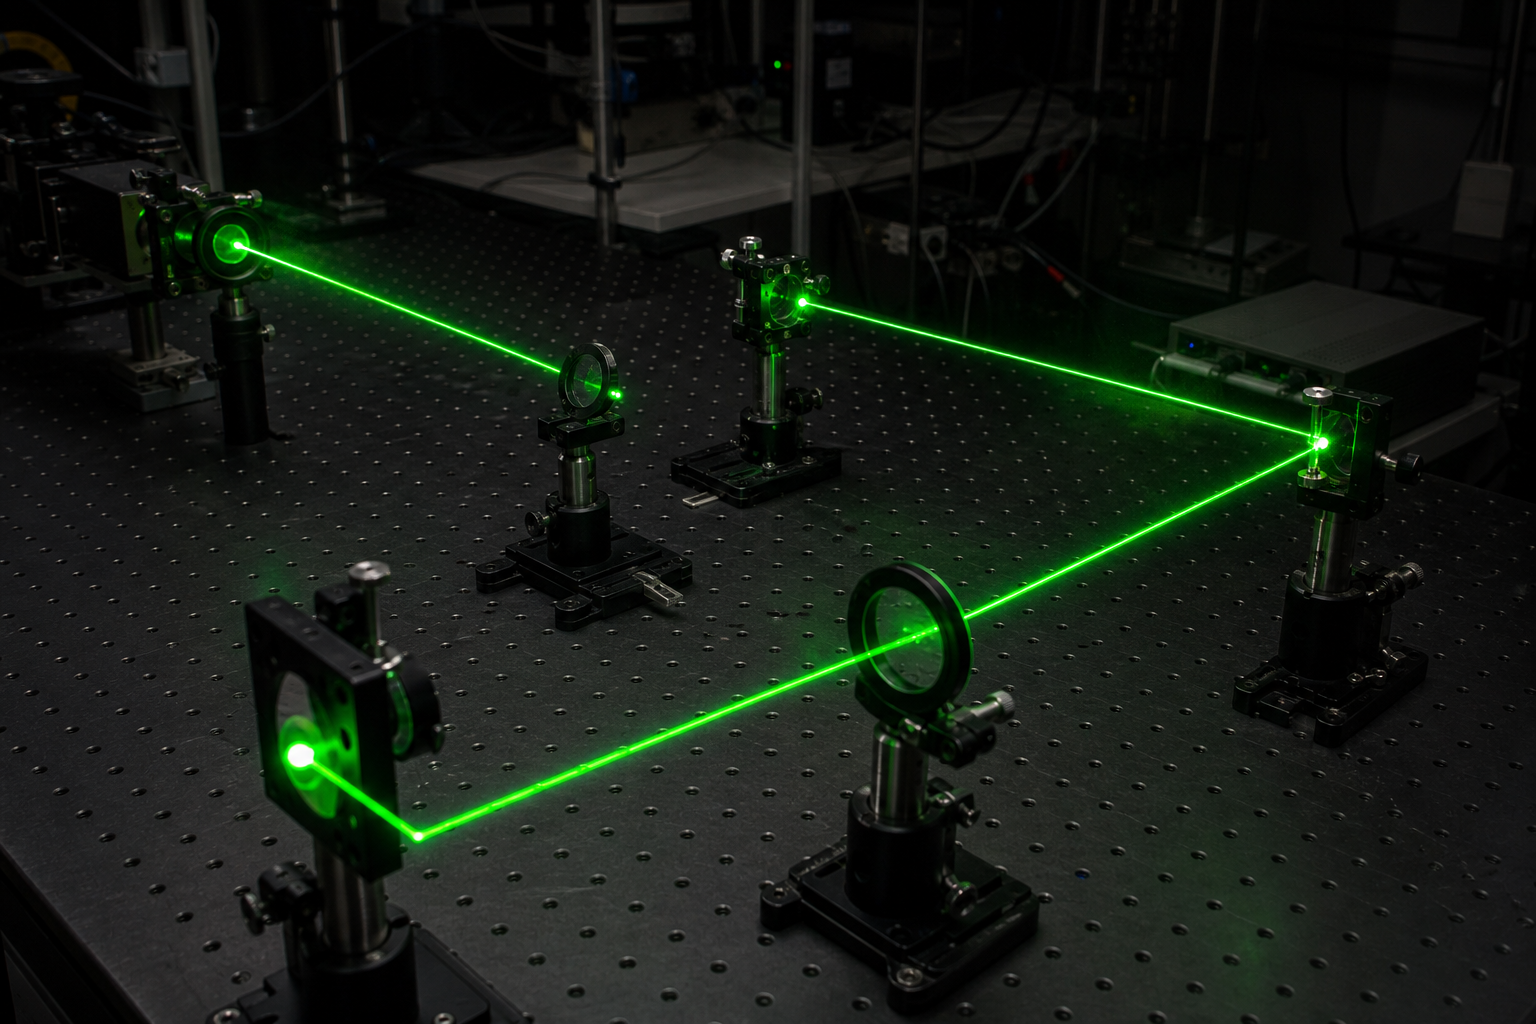
\includegraphics[width=0.58\linewidth]{images/book4/ai/b4-23-laser-optical-table.png}

{\small منضدة بصرية: \omterm{def:b2:laser:cavity}{ليزر}، ومرايا، وعدسات، وحزمة تبقى
خطًّا رفيعًا عبر الغرفة كلها --- وهي التوجيهية التي لا يعطيها
مصباح.}
\end{omfigure}

\section{الضوء والمادة: العمليات الثلاث}

\begin{definition}[الامتصاص والإصدار التلقائي والمستحثّ]\label{def:b2:laser:processes}
لتكن ذرات لها مستويا طاقة $E_1 < E_2$، وجمهرتاهما (أي كثافتا
العدد) $N_1$ و $N_2$، وضوء تواتره $\nu$ مع
$h\nu = E_2 - E_1$ وكثافة طاقة طيفية $u(\nu)$ (أي الطاقة في وحدة
الحجم ووحدة التواتر). وثلاث عمليات تتبادل الطاقة:
\begin{itemize}
\item \emph{الامتصاص}\index{الامتصاص (للضوء)}: ذرة في
      $E_1$ تمتصّ فوتونًا فترتفع إلى $E_2$، بالمعدل
      $B_{12}\,u(\nu)\,N_1$ في وحدة الحجم والزمن؛
\item \emph{الإصدار التلقائي}\index{إصدار تلقائي}: ذرة
      في $E_2$ تهبط إلى $E_1$ من تلقائها، فتصدر فوتونًا في جهة
      عشوائية وبطور عشوائي، بالمعدل $A_{21}N_2$ ---
      و $1/A_{21} = \tau$ هو عمر المستوي؛
\item \emph{الإصدار المستحثّ}\index{إصدار مستحثّ}: فوتون
      تواتره $\nu$ يمرّ بذرة في $E_2$ يحملها على الهبوط،
      فتصدر فوتونًا ثانيًا \emph{مطابقًا} للأول (أي التواتر
      نفسه والجهة والطور والاستقطاب)، بالمعدل
      $B_{21}\,u(\nu)\,N_2$.
\end{itemize}
و $A_{21}$ و $B_{12}$ و $B_{21}$ هي \emph{معاملات
أينشتاين}\index{معاملات أينشتاين} للانتقال.
\end{definition}

\begin{proposition}[علاقات أينشتاين]\label{prop:b2:laser:einstein}
من أجل مستويين غير منحلَّين،
\[
B_{12} = B_{21} \equiv B, \qquad
\frac{A_{21}}{B_{21}} = \frac{8\pi h\nu^3}{c^3}.
\]
فللإصدار المستحثّ \omterm{def:b2:laser:processes}{والامتصاص} المعامل نفسه؛ وينمو
المعدل التلقائي وفق $\nu^3$ بالنسبة إلى المعدل المستحثّ.
\end{proposition}

\begin{proof}
ضع الذرات في توازن مع الإشعاع عند الحرارة $T$. ونستعير
واقعتين من فصول لاحقة: نسبة جمهرتي
مستويين عند التوازن $N_2/N_1 = \eu^{-h\nu/k_BT}$ (أي
عامل بولتزمان، \cref{ch:b2:boltzmann-factor})، وللإشعاع
المتوازن كثافة بلانك الطيفية
$u(\nu) = (8\pi h\nu^3/c^3)/(\eu^{h\nu/k_BT} - 1)$
(\cref{ch:b2:thermal-radiation}). وعند التوازن تكون جمهرتا المستويين
مستقرتين: $B_{12}uN_1 = A_{21}N_2 + B_{21}uN_2$، ومن ثَمّ
\[
u = \frac{A_{21}}{B_{12}\,N_1/N_2 - B_{21}}
  = \frac{A_{21}}{B_{12}\eu^{h\nu/k_BT} - B_{21}}.
\]
ويجب أن يساوي هذا عبارة بلانك عند كل $T$: فحدّ $T \to \infty$
(حيث $u \to \infty$) يفرض $B_{12} = B_{21}$، وتعطي
المقارنة عندئذ $A_{21}/B_{21} = 8\pi h\nu^3/c^3$. والمعاملات
خواصّ للذرة، فالعلاقات صحيحة خارج
التوازن أيضًا.
\end{proof}

\begin{remark}[لمَ لا تضخّم المصابيح]\label{rem:b2:laser:lamps}
في غاز عند \qty{300}{K}، من أجل انتقال مرئي ($h\nu \approx
\qty{2}{eV}$، و $k_BT \approx \qty{0.025}{eV}$)، يكون $N_2/N_1 = \eu^{-80} \approx
10^{-35}$: أي لا ذرة مثارة عمليًّا، ولا يُمتصّ الضوء إلا امتصاصًا. والتفريغ
أو اللهب يعمر $E_2$، لكن مع $N_2 < N_1$ مع ذلك، وكل فوتون
مصدَر يغلبه عدد الامتصاصات؛ زد على ذلك أن نسبة
\omterm{def:b2:laser:processes}{الإصدار التلقائي} إلى المستحثّ عند التوازن،
$A_{21}/(B_{21}u) = \eu^{h\nu/k_BT} - 1$، كبيرة كِبَرًا فلكيًّا في
المرئي --- فضوء المصباح تلقائي: أطوار عشوائية، وجهات
كلها، وعرض الخط كاملًا. ولا ينافس \omterm{def:b2:laser:processes}{الإصدار المستحثّ}
طبيعيًّا إلا عند التواترات الراديوية والميكروية ($h\nu \ll k_BT$)؛
وقد كان أول جهاز من هذا النوع هو الميزر فعلًا، عند
\qty{24}{GHz} (1954)، قبل \omterm{def:b2:laser:cavity}{الليزر} الضوئي (1960).
\end{remark}

\begin{omfigure}
\begin{tikzpicture}[scale=0.9, >=stealth]
  \foreach \x/\t in {0/{الامتصاص}, 3.6/{الإصدار التلقائي}, 7.2/{الإصدار المستحثّ}}{
    \draw[thick] (\x,0) -- ++(2,0) node[right, font=\scriptsize] {$E_1$};
    \draw[thick] (\x,1.6) -- ++(2,0) node[right, font=\scriptsize] {$E_2$};
    \node[font=\scriptsize, align=center] at (\x+1,-0.5) {\t};
  }
  % absorption
  \fill (1,0) circle (2pt);
  \draw[->, omDef, thick] (1,0.15) -- (1,1.45);
  \draw[->, omExo, thick, decorate, decoration={snake, amplitude=0.6mm, segment length=2mm}] (-0.6,0.8) -- (0.7,0.8);
  \node[font=\scriptsize, omExo] at (-0.5,1.15) {$h\nu$};
  % spontaneous
  \fill (4.6,1.6) circle (2pt);
  \draw[->, omDef, thick] (4.6,1.45) -- (4.6,0.15);
  \draw[->, omExo, thick, decorate, decoration={snake, amplitude=0.6mm, segment length=2mm}] (4.8,0.8) -- (6.2,1.3);
  % stimulated
  \fill (8.2,1.6) circle (2pt);
  \draw[->, omDef, thick] (8.2,1.45) -- (8.2,0.15);
  \draw[->, omExo, thick, decorate, decoration={snake, amplitude=0.6mm, segment length=2mm}] (6.6,0.8) -- (7.9,0.8);
  \draw[->, omExo, thick, decorate, decoration={snake, amplitude=0.6mm, segment length=2mm}] (8.5,0.95) -- (9.9,0.95);
  \draw[->, omExo, thick, decorate, decoration={snake, amplitude=0.6mm, segment length=2mm}] (8.5,0.65) -- (9.9,0.65);
  \node[font=\scriptsize, omExo] at (10.6,0.8) {$2h\nu$};
\end{tikzpicture}

{\small العمليات الثلاث بين مستويين: \omterm{def:b2:laser:processes}{الامتصاص} يأخذ
فوتونًا؛ \omterm{def:b2:laser:processes}{والإصدار التلقائي} يضيف فوتونًا عشوائي الطور
والجهة؛ \omterm{def:b2:laser:processes}{والإصدار المستحثّ} يضيف فوتونًا مطابقًا للوارد
--- أي نسخة.}
\end{omfigure}

\section{التضخيم: انقلاب الجمهرة والربح}

\begin{proposition}[ربح وسط]\label{prop:b2:laser:gain}
حزمة شدتها $I$ عند التواتر $\nu$ تعبر الوسط
تكسب طاقة \omterm{def:b2:laser:processes}{بالإصدار المستحثّ} وتفقدها \omterm{def:b2:laser:processes}{بالامتصاص}
(\omterm{def:b2:laser:processes}{والإصدار التلقائي} يذهب في الجهات كلها ولا يكاد يسهم في
الحزمة). وعلى طول $\dd z$،
\[
\dd I = \sigma\,(N_2 - N_1)\,I\,\dd z, \qquad
I(z) = I(0)\,\eu^{g z}, \qquad g = \sigma(N_2 - N_1),
\]
حيث $\sigma$ (وهو مساحة، أي \emph{المقطع العرضي}\index{مقطع عرضي
(لانتقال)} للانتقال، $\sigma \propto B\,h\nu/c$) يقيس
شدة الانتقال. ولا \emph{يضخّم} الوسط ($g > 0$)
إلا إذا كان
\[
N_2 > N_1 :
\]
أي \emph{انقلاب جمهرة}\index{انقلاب الجمهرة}. ومن دونه
($N_2 < N_1$، وهي حال كل وسط عند التوازن) تُمتصّ
الحزمة.
\end{proposition}

\begin{proof}
في وحدة الحجم والزمن، تضيف $B u (N_2 - N_1)$ انتقالًا (أو تنزع)
فوتونًا $h\nu$ إلى الحزمة؛ ومع $u = I/c$ (في وحدة التواتر، على
عرض الخط)، تكون الاستطاعة المكتسبة في وحدة الحجم
$B h\nu (N_2 - N_1) I/c$، وهذه هي $\dd I/\dd z$؛ وعرّف $\sigma =
Bh\nu/c$ (مضروبًا في عامل شكل الخط).
\end{proof}

\begin{remark}[لمَ لا يمكن قلب مستويين]\label{rem:b2:laser:twolevel}
اضخخ نظامًا ذا مستويين ما شئت بضوء عند $\nu$: فالمضخّة
تُمتصّ حين $N_1 > N_2$ وتستحثّ الإصدار حين $N_2 > N_1$،
وتميل الجمهرتان في أحسن الأحوال إلى التساوي، $N_2 = N_1$، حيث يكون
الوسط شفافًا ولا يربح شيئًا. والانقلاب يحتاج إلى ثلاثة
مستويات على الأقل: فتُضخّ الذرات من المستوي الأساسي إلى مستوٍ قصير العمر
ينحلّ سريعًا إلى مستوي \omterm{def:b2:laser:cavity}{الليزر} الأعلى، وهو \emph{طويل العمر}
(شبه مستقر) فيخزن جمهرة. وفي المخطط
\emph{الثلاثي المستويات}\index{ليزر ثلاثي المستويات} (الياقوت، وهو أول
\omterm{def:b2:laser:cavity}{ليزر}) يكون مستوي \omterm{def:b2:laser:cavity}{الليزر} الأدنى هو الحالة الأساسية، فيجب رفع أكثر من نصف
الذرات قبل الانقلاب: فالمضخّة عنيفة. وفي المخطط
\emph{الرباعي المستويات}\index{ليزر رباعي المستويات} (هليوم--نيون، و Nd:YAG، ومعظم
الليزرات) يكون مستوي \omterm{def:b2:laser:cavity}{الليزر} الأدنى مستوًى مثارًا يفرغ سريعًا
إلى الحالة الأساسية؛ فهو شبه فارغ في كل حين، وجمهرة صغيرة
في المستوي الأعلى تكون انقلابًا أصلًا --- فالعتبة
منخفضة.
\end{remark}

\begin{omfigure}
\begin{tikzpicture}[scale=0.85, >=stealth]
  % ثلاثة مستويات
  \draw[thick] (0,0) -- (2,0) node[right, font=\scriptsize] {$0$: الأساسي};
  \draw[thick] (0,2.4) -- (2,2.4) node[right, font=\scriptsize] {$2$ (قصير العمر)};
  \draw[thick] (0,1.8) -- (2,1.8) node[right, font=\scriptsize] {$1$ (شبه مستقر)};
  \draw[->, omExo, thick] (0.5,0.05) -- (0.5,2.35) node[midway, left, font=\scriptsize] {مضخّة};
  \draw[->, dashed] (1.0,2.35) -- (1.0,1.85);
  \draw[->, omDef, very thick] (1.5,1.75) -- (1.5,0.05) node[midway, right, font=\scriptsize] {ليزر};
  \node[font=\scriptsize] at (1.8,-0.6) {ثلاثة مستويات (الياقوت)};
  % أربعة مستويات
  \begin{scope}[xshift=7cm]
  \draw[thick] (0,0) -- (2,0) node[right, font=\scriptsize] {$0$: الأساسي};
  \draw[thick] (0,2.4) -- (2,2.4) node[right, font=\scriptsize] {$3$ (قصير العمر)};
  \draw[thick] (0,1.9) -- (2,1.9) node[right, font=\scriptsize] {$2$ (شبه مستقر)};
  \draw[thick] (0,0.6) -- (2,0.6) node[right, font=\scriptsize] {$1$ (يفرغ سريعًا)};
  \draw[->, omExo, thick] (0.5,0.05) -- (0.5,2.35) node[midway, left, font=\scriptsize] {مضخّة};
  \draw[->, dashed] (1.0,2.35) -- (1.0,1.95);
  \draw[->, omDef, very thick] (1.5,1.85) -- (1.5,0.65) node[midway, right, font=\scriptsize] {ليزر};
  \draw[->, dashed] (1.0,0.55) -- (1.0,0.05);
  \node[font=\scriptsize] at (1.8,-0.6) {أربعة مستويات (هليوم--نيون، Nd:YAG)};
  \end{scope}
\end{tikzpicture}

{\small مخططا الضخّ. على اليسار: ثلاثة مستويات --- وانتقال \omterm{def:b2:laser:cavity}{الليزر}
ينتهي على المستوي الأساسي، الذي يجب إفراغ أكثر من نصفه. وعلى اليمين:
أربعة مستويات --- ومستوي \omterm{def:b2:laser:cavity}{الليزر} الأدنى ينزف فورًا إلى الحالة
الأساسية، فجمهرة عليا صغيرة تكون انقلابًا أصلًا.}
\end{omfigure}

\begin{proposition}[إشباع الربح]\label{prop:b2:laser:saturation}
يحفظ الانقلابَ مضخّةٌ تزوّد المستوي الأعلى بالذرات
بالمعدل $R$ في وحدة الحجم، في وجه الانحلال $1/\tau$
\omterm{def:b2:laser:processes}{والإصدار المستحثّ} $\sigma I (N_2 - N_1)/h\nu$. وفي وسط رباعي
المستويات ($N_1 \approx 0$) تكون الحالة المستقرة
\[
N_2 = \frac{R\tau}{1 + I/I_{\text{إشباع}}}, \qquad
g = \frac{g_0}{1 + I/I_{\text{إشباع}}}, \qquad
I_{\text{إشباع}} = \frac{h\nu}{\sigma\tau} :
\]
و\emph{الربح عند الإشارة الصغيرة} $g_0 = \sigma R\tau$ تخفضه الحزمة
نفسها متى اقترب $I$ من \emph{شدة
الإشباع}\index{شدة الإشباع} $I_{\text{إشباع}}$ --- فالمضخّم
لاخطي، وهذه اللاخطية هي التي ستثبّت استطاعة
\omterm{def:b2:laser:cavity}{الليزر}.
\end{proposition}

\begin{proof}
$\dd N_2/\dd t = R - N_2/\tau - \sigma I N_2/h\nu = 0$.
\end{proof}

\section{المذبذب: الجوف والعتبة والأنماط}

\begin{definition}[جوف الليزر]\label{def:b2:laser:cavity}
\emph{الليزر}\index{ليزر} وسط مضخّم طوله $\ell$
موضوع بين مرآتين (انعكاسيتاهما $R_1$ و $R_2$) تبعد إحداهما عن الأخرى $L$:
أي جوف فابري--بيرو (\cref{ch:b2:gratings}). وإحدى المرآتين، وهي
\emph{مقرِن الخرج}، نافذة جزئيًّا ($T_2 = 1 - R_2$ بضعة
في المئة) وتُخرج الحزمة. والضوء الذي يدور في الجوف
يُضخَّم مرتين بالوسط ويُوهَن بالمرآتين وبسائر
الضياعات (التبعثر \omterm{def:b2:laser:processes}{والامتصاص} \omterm{def:b2:diffraction:huygens}{والحيود}).
\end{definition}

\begin{theorem}[شرط التذبذب]\label{thm:b2:laser:threshold}
موجة سعتها العقدية $\underline s$ تعيد إنتاج نفسها بعد ذهاب
وإياب واحد إذا كان
\[
\underline s\,\cdot\, \eu^{g\ell}\sqrt{R_1}\,\eu^{g\ell}\sqrt{R_2}\,
\eu^{-\alpha\cdot 2L}\,\eu^{2\iu kL} = \underline s
\]
($\alpha$: سائر الضياعات في وحدة الطول). ومن ثَمّ شرطان.
\begin{itemize}
\item \emph{السعة}: $R_1R_2\,\eu^{2(g\ell - \alpha L)} \ge 1$، أي يجب أن يبلغ
      الربح \emph{العتبة}\index{عتبة (ليزر)}
      \[
      g_{\text{عتبة}} = \frac{1}{\ell}\Big(\alpha L - \tfrac12\ln(R_1R_2)\Big)
      \approx \frac{1}{2\ell}\,(T_2 + \text{الضياعات في الذهاب والإياب}) ;
      \]
\item \emph{الطور}: $2kL = 2\pi p$، أي $\nu_p = p\,c/2L$ --- فلا يتذبذب \omterm{def:b2:laser:cavity}{الليزر}
      إلا على \emph{الأنماط الطولية}\index{أنماط طولية}
      للجوف، المتباعدة $c/2L$، ولا إلا على ما يقع
      منها تحت منحني الربح حيث $g(\nu) \ge g_{\text{عتبة}}$.
\end{itemize}
\end{theorem}

\begin{proof}
يجب أن تكون سعة عامل الذهاب والإياب وطوره تافهتين معًا؛
والتقريب يستعمل $-\ln R \approx 1 - R = T$ من أجل $T \ll 1$.
\end{proof}

\begin{proposition}[الحالة المستقرة فوق العتبة]\label{prop:b2:laser:steady}
انطلاقًا من \omterm{def:b2:laser:processes}{الإصدار التلقائي} لذرة واحدة، ينمو كل نمط
$g_0 > g_{\text{عتبة}}$ فيه نموًّا أسّيًّا، ذهابًا وإيابًا بعد آخر؛
وكلما نمت شدته أشبع الربح
(\cref{prop:b2:laser:saturation}) حتى يساوي الضياعات بالضبط:
\[
g(I) = g_{\text{عتبة}} \quad\Longrightarrow\quad
I_{\text{جوف}} = I_{\text{إشباع}}\Big(\frac{g_0}{g_{\text{عتبة}}} - 1\Big),
\qquad P_{\text{خرج}} = T_2\,I_{\text{جوف}}\,A .
\]
فيُثبَّت الربح \emph{تثبيتًا} على قيمة العتبة؛ وكل ذرة زائدة
تُضَخّ فوق العتبة تصير فوتون خرج، فتنمو استطاعة الخرج
خطيًّا مع المضخّة فوق مضخّة العتبة.
\end{proposition}

\begin{remark}[الليزر مذبذب تغذية راجعة]\label{rem:b2:laser:feedback}
قارن \omterm{prop:b2:feedback-oscillators:wien}{بمذبذب جسر فين} في
\cref{ch:b2:feedback-oscillators}: مضخّم (وهو الوسط المقلوب)،
\omterm{def:b2:feedback-oscillators:loop}{وتغذية راجعة} انتقائية التواتر (وهي الجوف، الذي لا يمرّر إلا أنماطه)،
وشرط إقلاع (ربح الحلقة $> 1$، أي $g_0 > g_{\text{عتبة}}$)،
وإقلاع من الضجيج (وهو هنا \omterm{def:b2:laser:processes}{الإصدار التلقائي})، وسعة تثبّتها
لاخطية المضخّم (وهي إشباع الربح). \omterm{def:b2:laser:cavity}{فالليزر}
عضو الأسرة الضوئي.
\end{remark}

\begin{omfigure}
\begin{tikzpicture}
  \begin{axis}[omaxis, width=8.2cm, height=4.6cm, xmin=-2.4, xmax=2.4, ymin=0, ymax=1.25,
    xlabel={$(\nu - \nu_0)/\Delta\nu$}, ylabel={$g(\nu)$}, ytick=\empty,
    xtick={-2,-1,0,1,2}, clip=false]
    \addplot[omDef, thick, domain=-2.4:2.4, samples=120] {exp(-2.77*x*x)};
    \addplot[omExo, thick, dashed, domain=-2.4:2.4] {0.45};
    \node[font=\scriptsize, omExo, anchor=west] at (axis cs:1.6,0.55) {$g_{\text{th}}$};
    \draw[gray!70] (axis cs:-1.75,0) -- (axis cs:-1.75,0.12);
    \draw[gray!70] (axis cs:-1.4,0) -- (axis cs:-1.4,0.12);
    \draw[gray!70] (axis cs:-1.05,0) -- (axis cs:-1.05,0.12);
    \draw[gray!70] (axis cs:-0.7,0) -- (axis cs:-0.7,0.12);
    \draw[gray!70] (axis cs:0.7,0) -- (axis cs:0.7,0.12);
    \draw[gray!70] (axis cs:1.05,0) -- (axis cs:1.05,0.12);
    \draw[gray!70] (axis cs:1.4,0) -- (axis cs:1.4,0.12);
    \draw[gray!70] (axis cs:1.75,0) -- (axis cs:1.75,0.12);
    \draw[omThm, very thick] (axis cs:-0.35,0) -- (axis cs:-0.35,0.712);
    \draw[omThm, very thick] (axis cs:0,0) -- (axis cs:0,1.000);
    \draw[omThm, very thick] (axis cs:0.35,0) -- (axis cs:0.35,0.712);
    \node[font=\scriptsize, anchor=south] at (axis cs:-1.4,0.14) {$c/2L$};
    \draw[<->, thin] (axis cs:-1.75,0.12) -- (axis cs:-1.05,0.12);
  \end{axis}
\end{tikzpicture}

{\small منحني ربح الوسط (وعرضه $\Delta\nu$)، والعتبة
التي تضعها الضياعات، ومشط أنماط الجوف المتباعدة $c/2L$: فلا يتذبذب إلا
ما يقع تحت المنحني وفوق العتبة من الأنماط (وهي الغليظة).}
\end{omfigure}

\begin{example}[ليزر الهليوم--نيون]\label{ex:b2:laser:hene}
أنبوب زجاجي طوله \qty{30}{cm}، وتجويفه \qty{1}{mm}، فيه هليوم
ونيون عند نحو جزء من ألف من الجوّ، يعبره تفريغ
بضعة مليأمبيرات. وتثير الإلكترونات الهليوم إلى مستوٍ شبه مستقر عند
\qty{20.6}{eV}، وهو يسلّم طاقته بالتصادم إلى مستوي نيون على
الارتفاع نفسه تقريبًا؛ ومن هناك ينحلّ النيون إلى مستوٍ أدنى
(يفرغ سريعًا إلى الحالة الأساسية --- أي رباعي المستويات) بالإصدار عند
\qty{632.8}{nm}. والربح عند الإشارة الصغيرة ضئيل، بضعة في المئة في كل
مرور، فيجب أن تكون المرآتان ممتازتين ($R_1 = 0.999$، و $R_2 = 0.99$)
والأنبوب نظيفًا؛ وخط الربح معرَّض دوبلريًّا إلى
$\Delta\nu \approx \qty{1.5}{GHz}$، والأنماط متباعدة $c/2L = \qty{500}{MHz}$،
فيتذبذب نمطان أو ثلاثة معًا. والخرج \qty{1}{mW} من أجل
عدة واطات من التفريغ: أي مردود $10^{-4}$؛ لكن بطول موجة
معيَّن حتى $10^{-6}$ وحزمة تبقى بعرض \qty{1}{mm} عبر
المخبر.
\end{example}

\section{الحزمة الغاوسية}

\begin{proposition}[الحزمة الغاوسية]\label{prop:b2:laser:gaussian}
الحزمة التي يصدرها جوف مستقر ذو مرآتين محدّبتين هي (في
النمط المستعرض الأساسي) \emph{حزمة غاوسية}\index{حزمة
غاوسية}: فعلى البعد $z$ عن أضيق مقاطعها (أي
\emph{الخصر}\index{خصر (حزمة)}، ونصف قطره $w_0$) يكون مقطع
الشدة
\[
I(r,z) = \frac{2P}{\pi w(z)^2}\,\exp\Big(-\frac{2r^2}{w(z)^2}\Big),
\qquad
w(z) = w_0\sqrt{1 + \Big(\frac{z}{z_{\text{R}}}\Big)^2},
\qquad
z_{\text{R}} = \frac{\pi w_0^2}{\lambda},
\]
حيث $P$ الاستطاعة الكلية و $z_{\text{R}}$ \emph{طول
رايلي}\index{طول رايلي}: فعلى $\pm z_{\text{R}}$ تبقى الحزمة
ضمن $\sqrt2$ من خصرها، وفي ما وراءه بكثير تنتشر بنصف
الزاوية
\[
\theta = \frac{\lambda}{\pi w_0} .
\]
والحزمة حلّ \omterm{thm:b2:waves-on-strings:equation}{لمعادلة الأمواج} في التقريب
المحوري القريب؛ ونقبل شكلها ونستعمله. وجبهات موجتها مستوية عند
\omterm{prop:b2:laser:gaussian}{الخصر} وكروية بعيدًا.
\end{proposition}

\begin{proof}
مقبول في هذا المستوى (والحساب هو انتشار توزيع فتحة غاوسية
في بصريات فورييه)؛ وخاصّته الأساسية هي
التي أعطاها \omterm{def:b2:diffraction:huygens}{الحيود} أصلًا في \cref{ch:b2:diffraction}: فالفتحة
التي حجمها $w_0$ تنتشر على $\lambda/w_0$، وهنا بالعامل المضبوط
$1/\pi$.
\end{proof}

\begin{omfigure}
\begin{tikzpicture}
  \begin{axis}[omaxis, width=9cm, height=4.6cm, xmin=-3.2, xmax=3.2, ymin=-3.4, ymax=3.4,
    xlabel={$z/z_{\text{R}}$}, ylabel={$r/w_0$}, clip=false, xtick={-3,-2,-1,0,1,2,3}, ytick={-2,-1,1,2}]
    \addplot[omDef, thick, domain=-3.2:3.2, samples=100] {sqrt(1+x*x)};
    \addplot[omDef, thick, domain=-3.2:3.2, samples=100] {-sqrt(1+x*x)};
    \addplot[omExo, dashed, domain=-3.2:3.2] {x};
    \addplot[omExo, dashed, domain=-3.2:3.2] {-x};
    \draw[<->, thin] (axis cs:0.3,-1.04) -- (axis cs:0.3,1.04) node[pos=0.25, right, font=\scriptsize] {$2w_0$};
    \node[font=\scriptsize, omExo, anchor=north west] at (axis cs:0.8,3.5) {$\theta = \lambda/\pi w_0$};
  \end{axis}
\end{tikzpicture}

{\small \omterm{prop:b2:laser:gaussian}{حزمة غاوسية}: نصف القطر $w(z)$ قطع زائد --- شبه
ثابت ضمن \omterm{prop:b2:laser:gaussian}{طول رايلي}، ثم مخروط نصف زاويته
$\lambda/\pi w_0$. وخصر أصغر يعني \omterm{prop:b2:laser:gaussian}{طول رايلي} أقصر ومخروطًا
أوسع.}
\end{omfigure}

\begin{proposition}[تجميع حزمة وتوسيعها]\label{prop:b2:laser:focus}
\omterm{prop:b2:laser:gaussian}{حزمة غاوسية} نصف قطرها $w$ (أكبر بكثير مما كان يعطيه حقلها
البعيد عند العدسة، أي شبه موازية) تقع على عدسة بعدها
البؤري $f$ تُجمَّع في خصر
\[
w_0' = \frac{\lambda f}{\pi w}
\]
عند البؤرة، \omterm{prop:b2:laser:gaussian}{وطول رايلي} فيه $\pi w_0'^2/\lambda$. وذروة
الاستضاءة هناك $2P/\pi w_0'^2$. وبالعكس يحوّل مقراب لابؤري
تكبيره $M$ حزمة نصف قطرها $w$ إلى حزمة نصف قطرها $Mw$
تفرّجها أصغر بالعامل $M$: فلترسل حزمة بعيدًا، اجعلها
أولًا عريضة.
\end{proposition}

\begin{proof}
تحوّل العدسة \omterm{def:b2:scalar-light-model:path}{جبهة الموجة} المستوية إلى كرة متقاربة عند $f$؛
\omterm{def:b2:diffraction:huygens}{وحيود} فتحة نصف قطرها $w$ يعطي الانتشار الزاوي
$\lambda/\pi w$، ومن ثَمّ البقعة البؤرية $f\lambda/\pi w$ --- وهو متوافق مع
$\theta = \lambda/\pi w_0'$ مقروءًا بالمقلوب.
\end{proof}

\begin{example}[القطع والقراءة والتأشير]\label{ex:b2:laser:focus}
\omterm{def:b2:laser:cavity}{ليزر} ثنائي أكسيد الكربون \qty{1}{kW} عند \qty{10.6}{\micro m}، ونصف قطر حزمته
\qty{10}{mm}، مجمَّعًا بعدسة $f = \qty{100}{mm}$: $w_0' = \qty{34}{\micro m}$،
وذروة الاستضاءة $2P/\pi w_0'^2 = \qty{5e11}{W/m^2}$ --- فيغلي الفولاذ.
ومؤشر \qty{1}{mW}، $w_0 = \qty{0.5}{mm}$ عند \qty{633}{nm}: $\theta =
\qty{0.4}{mrad}$، أي بقعة \qty{4}{cm} على \qty{50}{m}، واستضاءة
\qty{2.5}{kW/m^2} عند المخرج --- أي فوق ضوء الشمس، ولهذا يجب ألا يدخل
حتى المليواط عينًا: إذ تجمّعه عدسة العين في بقعة
\qty{10}{\micro m} على الشبكية بملايين الواطات في المتر
المربع. وقارئ قرص عند \qty{650}{nm} بعدسة فتحتها العددية
$0.6$ يجمّع في نحو $\lambda/2\mathrm{NA} \approx \qty{0.5}{\micro m}$،
أي حجم حفرة.
\end{example}

\begin{remark}[ما الذي يميّز ضوء الليزر]\label{rem:b2:laser:special}
\emph{التوجيهية}: نمط مستعرض واحد، وتفرّج عند حدّ
\omterm{def:b2:diffraction:huygens}{الحيود}. و\emph{أحادية اللون}: نمط جوف واحد أو بضعة، وكل منها
أضيق من ميغاهرتز --- أي أطوال ترابط بالأمتار إلى الكيلومترات
(\cref{ch:b2:scalar-light-model}). و\emph{\omterm{prop:b2:two-wave-interference:spatial}{الترابط المكاني}}: فالحزمة
كلها موجة واحدة، فتتداخل مع نفسها في أي مكان (وهو التصوير المجسّم،
وقياس التداخل). و\emph{السطوع}: فمليواط في حزمة محدودة
\omterm{def:b2:diffraction:huygens}{بالحيود} يفوق الشمس في وحدة الزاوية المجسمة وعرض النطاق. و\emph{الاستطاعة}
في النبضات: فجول في نانوثانية غيغاواط، وفي فمتوثانية
بيتاواط. ولأن الحزمة خرج مذبذب، يمكن
تعديلها عند الغيغاهرتز --- وهي حاملة \omterm{prop:b2:guided-waves:fibre}{الليف البصري}
(\cref{ch:b2:guided-waves}).
\end{remark}

\begin{method}[تقديرات الليزر]\label{meth:b2:laser:method}
(1) طاقة الفوتون $h\nu = hc/\lambda$ ومعدل الفوتونات $P/h\nu$.
(2) والعتبة: $g_{\text{عتبة}}\ell \approx \tfrac12(T_2 + \text{الضياعات})$؛
وقارنها بربح الوسط عند الإشارة الصغيرة $g_0\ell$.
(3) والأنماط: $c/2L$ في وجه عرض الربح؛ وعُدّ الأنماط المتذبذبة.
(4) والاستطاعة: يثبت الربح عند العتبة؛ والخرج $\propto$ (المضخّة $-$
مضخّة العتبة). (5) والحزمة: $z_{\text{R}} = \pi w_0^2/\lambda$، و $\theta =
\lambda/\pi w_0$، والبقعة البؤرية $\lambda f/\pi w$، وذروة الاستضاءة
$2P/\pi w_0^2$. (6) والسلامة: قارن استضاءة الشبكية باستضاءة
الشمس.
\end{method}

\section{تمارين}

\begin{exercise}[$\star$]\label{exo:b2:laser:1}
\omterm{def:b2:laser:cavity}{ليزر} هليوم--نيون يصدر \qty{1}{mW} عند \qty{632.8}{nm}. أوجد التواتر، وطاقة
الفوتون بالجول وبالإلكترون فولت، والفوتونات في الثانية. والجوف
\qty{30}{cm}: أوجد \omterm{def:b2:maxwell-equations:operators}{تباعد} الأنماط؛ وكم نمطًا يسع تحت منحني ربح
عرضه \qty{1.5}{GHz}؟
\end{exercise}

\begin{exercise}[$\star$]\label{exo:b2:laser:2}
مستويان يبعد أحدهما عن الآخر \qty{2}{eV} عند \qty{300}{K}: أوجد النسبة $N_2/N_1$ (استعمل
$k_BT = \qty{0.025}{eV}$). وعند أي حرارة تتساوى الجمهرتان؟
وبيّن أن الانقلاب يقابل حرارة \emph{سالبة} صوريًّا
في نسبة بولتزمان. وأعد النسبة نفسها من أجل انتقال ميكروي
عند \qty{24}{GHz}.
\end{exercise}

\begin{exercise}[$\star$]\label{exo:b2:laser:3}
\omterm{prop:b2:laser:gaussian}{حزمة غاوسية}، $w_0 = \qty{0.5}{mm}$، و $\lambda = \qty{633}{nm}$: أوجد \omterm{prop:b2:laser:gaussian}{طول
رايلي}، والتفرّج، ونصف القطر بعد \qty{100}{m} وعند القمر
(\qty{3.8e8}{m}). وأعد ذلك للحزمة نفسها بعد موسّع $\times 20$.
\end{exercise}

\begin{exercise}[$\star$]\label{exo:b2:laser:4}
جوف مع $R_1 = 1$، و $R_2 = 0.98$، ووسط طوله \qty{20}{cm}، وسائر
الضياعات $0.5\%$ في المرور. أوجد معامل ربح العتبة. وربح الوسط
عند الإشارة الصغيرة \qty{0.2}{m^{-1}}: أيتذبذب؟ ومع
$R_2 = 0.90$؟
\end{exercise}

\begin{exercise}[$\star\star$]\label{exo:b2:laser:5}
\emph{علاقات أينشتاين.} (أ) اكتب موازنة جمهرة
مستويين في توازن مع إشعاع $u(\nu)$ واستنتج العلاقتين
من قانون بلانك (المعطى). (ب) واحسب
$A_{21}/B_{21}u = \eu^{h\nu/k_BT} - 1$ عند \qty{300}{K} من أجل
$\lambda = \qty{600}{nm}$ ومن أجل $\lambda = \qty{1}{cm}$. (ج) ولمَ اخْتُرع
الميزر قبل \omterm{def:b2:laser:cavity}{الليزر}؟ (د) وعمر المستوي هو
$\tau = 1/A_{21}$؛ فإذا كان $\tau = \qty{10}{ns}$ عند \qty{600}{nm}، فما
$\tau$ من أجل انتقال له $B$ نفسه عند \qty{6}{\micro m}؟
\end{exercise}

\begin{exercise}[$\star\star$]\label{exo:b2:laser:6}
\emph{الإشباع واستطاعة الخرج.} وسط رباعي المستويات، $\sigma =
\qty{3e-17}{m^2}$، و $\tau = \qty{100}{ns}$، و $\lambda = \qty{633}{nm}$.
(أ) أوجد \omterm{prop:b2:laser:saturation}{شدة الإشباع}. (ب) ومعدل الضخّ $R$ من أجل ربح عند إشارة صغيرة
$g_0 = \qty{0.1}{m^{-1}}$. (ج) وعتبة الجوف
$g_{\text{عتبة}} = \qty{0.02}{m^{-1}}$: أوجد الشدة داخل الجوف في الحالة
المستقرة؛ والخرج عبر $T_2 = 1\%$ من حزمة مساحتها \qty{1}{mm^2}.
(د) وبيّن أن استطاعة الخرج خطية في $R$ فوق العتبة.
\end{exercise}

\begin{exercise}[$\star\star$]\label{exo:b2:laser:7}
\emph{الأنماط والاستقرار.} (أ) أوجد طول الجوف من أجل تشغيل أحادي النمط
تحت منحني ربح \qty{1.5}{GHz}. (ب) وجوف \qty{30}{cm} يتمدد
\qty{1}{\micro m}: أوجد انزياح تواتر نمط، مقارنًا \omterm{def:b2:maxwell-equations:operators}{بتباعد}
الأنماط وبعرض الربح. (ج) ولمَ تثبّت ليزرات هليوم--نيون
التجارية المستقرة طولَ الأنبوب بتسخينه؟ (د) وعرض النمط نفسه
بضعة كيلوهرتزات: فما \omterm{prop:b2:scalar-light-model:coherence}{طول الترابط}؟
\end{exercise}

\begin{exercise}[$\star\star$]\label{exo:b2:laser:8}
\emph{التجميع.} (أ) حزمة $w = \qty{1}{mm}$، و $\lambda = \qty{633}{nm}$،
و $f = \qty{50}{mm}$: أوجد \omterm{prop:b2:laser:gaussian}{الخصر}، \omterm{prop:b2:laser:gaussian}{وطول رايلي}، وذروة الاستضاءة من أجل
\qty{1}{mW}. (ب) والحزمة نفسها في عين (بعدها البؤري \qty{17}{mm}):
أوجد البقعة الشبكية والاستضاءة؛ وقارنهما بصورة الشمس
(\qty{1}{kW/m^2} عبر بؤبؤ \qty{3}{mm} في صورة \qty{0.15}{mm}).
(ج) ولمَ يكون مؤشر أخضر \qty{5}{mW} أخطر من
مصباح \qty{100}{W}؟ (د) وعمق تجميع عدسة \qty{50}{mm}.
\end{exercise}

\begin{exercise}[$\star\star$]\label{exo:b2:laser:9}
\emph{ثلاثة مستويات مقابل أربعة.} الياقوت: $N = \qty{1.6e25}{m^{-3}}$
شاردة كروم، وعمر المستوي الأعلى \qty{3}{ms}، و $\lambda =
\qty{694}{nm}$. (أ) أوجد أصغر استطاعة ضخّ في وحدة الحجم لإبقاء نصف
الشوارد في المستوي الأعلى. (ب) ومن أجل قضيب \qty{1}{cm^3}. (ج) والوسط الرباعي
المستويات لا يحتاج إلا إلى $\Delta N = \qty{1e22}{m^{-3}}$ مع $\tau =
\qty{230}{\micro s}$ عند \qty{1064}{nm}: أوجد استطاعة الضخّ في وحدة الحجم. (د) وعلّق
على مصباح وميض \omterm{def:b2:laser:cavity}{ليزر} الياقوت في مقابل الضخّ بالثنائيات في Nd:YAG.
\end{exercise}

\begin{exercise}[$\star\star\star$]\label{exo:b2:laser:10}
\emph{الثنائي الليزري.} منطقة الإصدار في ثنائي ليزري نحو
\qty{3}{\micro m} في \qty{1}{\micro m}، و $\lambda = \qty{780}{nm}$. (أ)
أوجد نصفي زاويتي التفرّج في الجهتين. (ب) وأي جهة
تتفرّج أكثر، ولمَ تكون الحزمة إهليلجية؟ (ج) وعدسة $f =
\qty{5}{mm}$ توازيها: أوجد حجمي الحزمة في الجهتين. (د) وكيف
يمكن جعل الإهليلج دائريًّا (فكرتان)؟
\end{exercise}

\begin{exercise}[$\star\star\star$]\label{exo:b2:laser:11}
\emph{الإقلاع.} (أ) اكتب شرط سعة الذهاب والإياب مع
ربح صافٍ $G = \eu^{2(g_0 - g_{\text{عتبة}})\ell} = 1.04$ في الذهاب والإياب
وزمن ذهاب وإياب $2L/c$ مع $L = \qty{30}{cm}$. (ب) ومن فوتون
تلقائي واحد إلى الحالة المستقرة \qty{100}{mW} داخل الجوف
(فكم عدد الفوتونات في الجوف؟)، كم مرة ذهابًا وإيابًا وكم من الزمن؟
(ج) وما الذي يحدّ النمو، وماذا يحلّ بنمط يكون فيه
$g_0 < g_{\text{عتبة}}$؟ (د) وفي \omterm{def:b2:laser:cavity}{ليزر} متعدد الأنماط تتنافس الأنماط على
الذرات نفسها: فسّر قفز الأنماط.
\end{exercise}

\begin{exercise}[$\star\star\star$]\label{exo:b2:laser:12}
\emph{قياس مدى القمر.} نبضات \qty{100}{mJ} عند \qty{532}{nm}،
ومدتها \qty{100}{ps}، تُرسَل عبر مقراب \qty{1}{m} ($w_0 =
\qty{0.5}{m}$). (أ) أوجد الفوتونات في النبضة، وذروة الاستطاعة. (ب) وتفرّج
\omterm{def:b2:diffraction:huygens}{الحيود} ونصف قطر البقعة على القمر (\qty{3.8e8}{m})؛ والجوّ
ينشر الحزمة إلى \qty{1}{''} بدل ذلك: أوجد نصف قطر البقعة. (ج) ورصّة
عاكسات مساحتها \qty{0.1}{m^2} على القمر تعيد الضوء بحيودها
هي ($\lambda/d$ مع مكعبات ركنية $d = \qty{4}{cm}$): أوجد البقعة على
الأرض، والنسبة التي يلتقطها المقراب، والفوتونات المكشوفة في النبضة.
(د) والتوقيت حتى \qty{100}{ps}: أوجد دقة المسافة في النبضة، وبعد
$10^4$ نبضة.
\end{exercise}

\begin{omfigure}
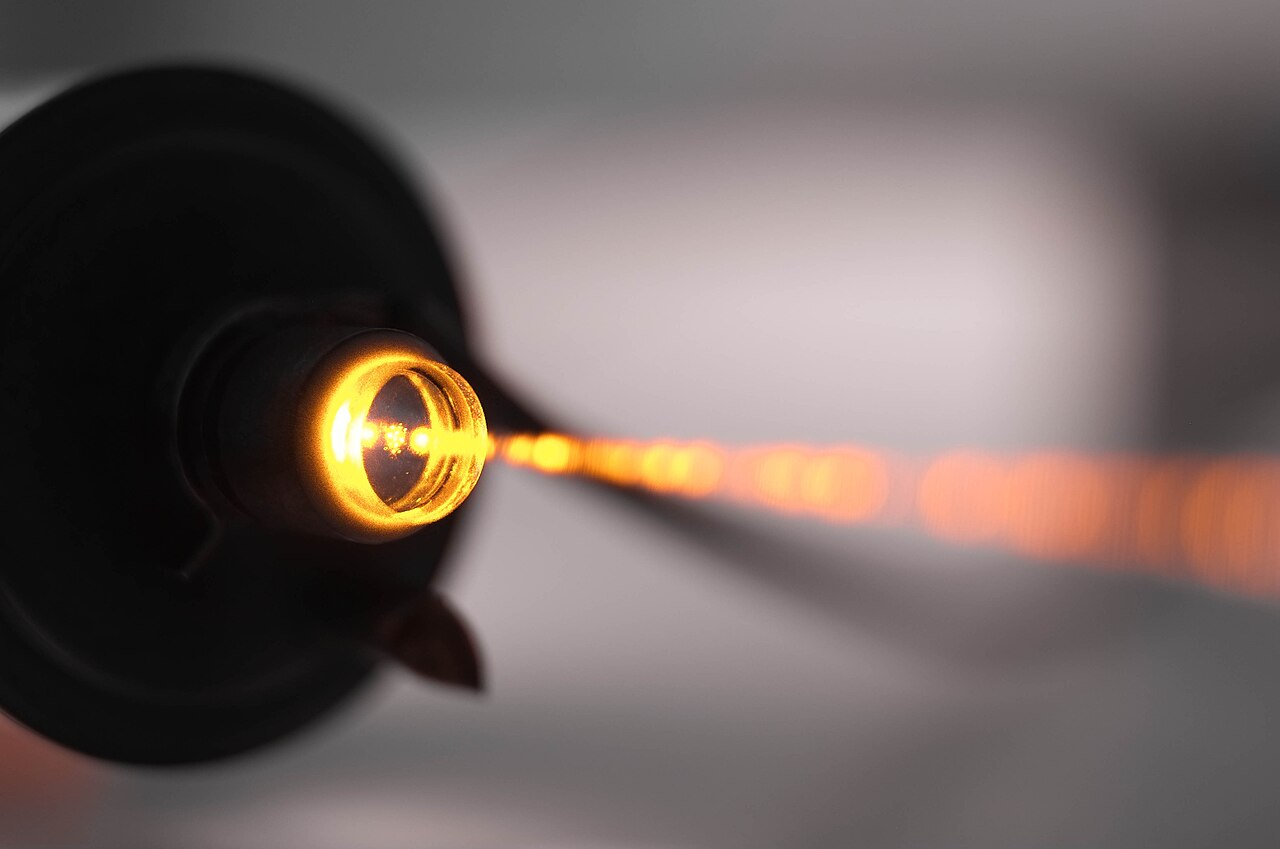
\includegraphics[width=0.58\linewidth]{images/book4/hene-laser-594nm.jpg}

{\small أنبوب \omterm{def:b2:laser:cavity}{ليزر} هليوم--نيون يصدر على خطه الأصفر عند \qty{594}{nm}: توهج التفريغ داخل الأنبوب، والحزمة الخارجة عبر مرآة الخرج. الصورة: تيليمنتور، CC~BY~4.0.}
\end{omfigure}

\section{مسألة: ليزر هليوم--نيون، من الأنبوب إلى القمر}

\begin{problem}[{مسألة نهاية الأسبوع --- ليزر يُبنى ويُوصَف
ويُستعمل}]\label{pb:b2:laser:1}
\omterm{def:b2:laser:cavity}{الليزر} على المنضدة: أنبوب زجاجي $L = \qty{30}{cm}$، وقطر تجويفه
\qty{1}{mm}، ومزيج هليوم ونيون، وتفريغ \qty{5}{mA} تحت
\qty{1.5}{kV}؛ ومرآتان $R_1 = 0.999$ و $R_2 = 0.99$؛ وطول الموجة
\qty{632.8}{nm}؛ والخرج \qty{1}{mW}. والمعطيات: مستوي الهليوم شبه المستقر يقع
عند \qty{20.61}{eV}، ومستوي \omterm{def:b2:laser:cavity}{الليزر} الأعلى للنيون عند \qty{20.66}{eV} وعمره
\qty{100}{ns}، ومستوي \omterm{def:b2:laser:cavity}{الليزر} الأدنى عند \qty{18.70}{eV} وعمره
\qty{10}{ns}؛ وحرارة الغاز \qty{400}{K}؛ والكتلة المولية للنيون
\qty{20}{g/mol}؛ \omterm{prop:b2:laser:gain}{والمقطع العرضي} $\sigma = \qty{3e-17}{m^2}$؛ و $h =
\qty{6.63e-34}{J.s}$، و $k_B = \qty{1.38e-23}{J/K}$، و $k_BT$ عند \qty{400}{K}
$= \qty{0.0345}{eV}$.

\textbf{الجزء الأول --- الوسط.}
\begin{enumerate}
  \item أوجد طاقة الفوتون وتواتر خط \omterm{def:b2:laser:cavity}{الليزر}.
  \item ومستويا الهليوم والنيون يختلفان بمقدار \qty{0.05}{eV}: قارن ذلك بالمقدار
        $k_BT$ وفسّر لمَ يكون نقل التصادم هليوم $\to$ نيون
        فعّالًا.
  \item ونسبة بولتزمان لمستوي النيون الأعلى إلى الحالة الأساسية عند
        \qty{400}{K} من دون تفريغ: علّق.
  \item وفسّر، من العمرين، لمَ يسهل حفظ انقلاب بين
        مستويي النيون متى غُذّي المستوي الأعلى.
  \item وعرض دوبلر للخط: أوجد السرعة الأرجح للنيون عند
        \qty{400}{K} و $\Delta\nu \approx \nu\,v/c$ من حيث رتبة
        المقدار (وبالضبط $\Delta\nu = 2\nu\sqrt{2k_BT\ln2/Mc^2}$).
  \item ومع $\Delta N = N_2 - N_1 = \qty{3e15}{m^{-3}}$: أوجد معامل الربح
        عند الإشارة الصغيرة والربح في المرور على \qty{30}{cm}.
\end{enumerate}

\textbf{الجزء الثاني --- الجوف.}
\begin{enumerate}[resume]
  \item أوجد معامل ربح العتبة؛ والهامش بالنسبة إلى السؤال 6.
  \item \omterm{def:b2:maxwell-equations:operators}{وتباعد} الأنماط؛ وعدد الأنماط التي يمكن أن تتذبذب.
  \item والاستطاعة داخل الجوف والاستضاءة داخل الجوف في التجويف.
  \item وما الذي يثبّت الربح في الحالة المستقرة، وأين تذهب طاقة
        الضخّ الزائدة؟
  \item والاستطاعة الكهربائية الداخلة والاستطاعة الضوئية الخارجة: أوجد المردود؛
        وسببين لكونه منخفضًا إلى هذا الحدّ.
  \item والإقلاع: أوجد الربح الصافي في الذهاب والإياب $2(g_0 - g_{\text{عتبة}})L$،
        وعدد الفوتونات في الجوف في الحالة المستقرة، وعدد
        مرات الذهاب والإياب من فوتون واحد، وزمن الإقلاع.
  \item ويسخن الأنبوب فيطول \qty{1}{\micro m}: أوجد انزياح
        تواتر نمط؛ والنتيجة من أجل \omterm{def:b2:laser:cavity}{ليزر} أحادي النمط.
  \item والأنبوب مغلق بنافذتين عند \omterm{prop:b2:wave-interfaces:brewster}{زاوية بروستر}: فماذا يفعل
        ذلك باستقطاب الخرج، ولمَ لا يضيف
        ضياعًا؟
\end{enumerate}

\textbf{الجزء الثالث --- الحزمة.}
\begin{enumerate}[resume]
  \item ينتج الجوف خصرًا $w_0 = \qty{0.3}{mm}$: أوجد \omterm{prop:b2:laser:gaussian}{طول
        رايلي}، والتفرّج، وقطر الحزمة على بعد \qty{10}{m}.
  \item وذروة الاستضاءة عند المخرج؛ وقارنها بضوء الشمس
        (\qty{1}{kW/m^2}).
  \item وعدسة $f = \qty{50}{mm}$: أوجد \omterm{prop:b2:laser:gaussian}{الخصر} وذروة الاستضاءة عند
        البؤرة.
  \item وتدخل الحزمة عينًا (بعدها البؤري \qty{17}{mm}): أوجد البقعة الشبكية
        والاستضاءة؛ ولمَ لا تكون الرمشة أبطأ من اللازم من أجل \qty{1}{mW}،
        وما معنى ``الصنف 2''.
  \item وموسّع حزمة $\times 10$: أوجد التفرّج الجديد وقطر البقعة
        على \qty{1}{km}.
  \item \omterm{prop:b2:scalar-light-model:coherence}{وطول الترابط} إذا عمل \omterm{def:b2:laser:cavity}{الليزر} على نمط واحد عرضه
        \qty{1}{MHz}؛ وإذا عمل على ثلاثة أنماط تمتد على \qty{1}{GHz}.
\end{enumerate}

\textbf{الجزء الرابع --- إلى القمر.}
محطة قياس مدى تطلق نبضات \qty{100}{mJ} مدتها \qty{100}{ps} عند
\qty{532}{nm} عبر مقراب \qty{1}{m}؛ والجوّ ينشر
الحزمة الخارجة إلى \qty{1}{''} ($\qty{4.8e-6}{rad}$).
\begin{enumerate}[resume]
  \item أوجد الفوتونات في النبضة وذروة الاستطاعة.
  \item ونصف قطر البقعة على القمر (\qty{3.8e8}{m})؛ وقارنه بالبقعة
        المحدودة \omterm{def:b2:diffraction:huygens}{بالحيود}.
  \item ورصّة عاكسات مساحتها \qty{0.1}{m^2} تعترض أي نسبة من
        النبضة، وكم فوتونًا؟
  \item والمكعبات الركنية \qty{4}{cm} في الرصّة تعيد الضوء
        بالانتشار $\lambda/d$: أوجد نصف قطر البقعة على الأرض، والنسبة التي يلتقطها
        المقراب، والفوتونات المكشوفة في النبضة (خذ مردودًا بصريًّا
        كليًّا $0.1$).
  \item وزمن الذهاب والإياب نحو \qty{2.56}{s}، مقيسًا حتى
        \qty{100}{ps}: أوجد دقة المسافة في النبضة؛ وبعد $10^4$
        عودة؛ وقارنها بمقدار \qty{3.8}{cm} في السنة التي يبتعد بها
        القمر.
\end{enumerate}
\end{problem}
